% Gemini theme
% https://github.com/anishathalye/gemini
\documentclass[final]{beamer}
\listfiles
% ====================
% Packages
% ====================

\usepackage[T1]{fontenc}
\usepackage{lmodern}
\usepackage[size=a0,scale=1]{beamerposter}
\usetheme{gemini}
\usecolortheme{IC}
\usepackage{graphicx}
\usepackage{booktabs}
\usepackage{tikz}
\usepackage{tikz-cd}
\usepackage[backend=bibtex,style=numeric,maxnames=2, minnames=2]{biblatex}
\addbibresource{refs.bib}


\AtEveryBibitem{
	\clearfield{month}
	\clearfield{series}
	\clearfield{venue}
	\clearname{editor}
	\clearlist{publisher}
	\clearlist{location} % alias to field 'address'
	\clearfield{doi}
	\clearfield{url}
	\clearfield{venue}
	\clearfield{issn}
	\clearfield{isbn}
	\clearfield{urldate}
	\clearfield{eventdate}
	\clearfield{pages}
	\clearfield{booktitle}
	\clearfield{journaltitle}
	\clearfield{number}
	\clearfield{volume}
}



% ====================
% Lengths
% ====================

% If you have N columns, choose \sepwidth and \colwidth such that
% (N+1)*\sepwidth + N*\colwidth = \paperwidth
\newlength{\sepwidth}
\newlength{\colwidth}
\setlength{\sepwidth}{0.00\paperwidth}
\setlength{\colwidth}{0.19\paperwidth}

\newcommand{\separatorcolumn}{\begin{column}{\sepwidth}\end{column}}

% ====================
% Title
% ====================

\title{Minimal Models in Mixed Characteristic}

\author{Liam Stigant}

\institute[shortinst]{Imperial College London}


% ====================
% Footer (optional)
% ====================

\footercontent{
	22/09/22 \hfill Algebraic Geometry in Cetraro 2021 together with Ciro Ciliberto \hfill
	\href{mailto:l.stigant18@imperial.ac.uk}{L.Stigant18@imperial.ac.uk}}
% (can be left out to remove footer)


% ====================
% Body
% ====================

\begin{document}
	
	\begin{frame}[t, fragile]
	\begin{columns}[t]
		\separatorcolumn
		
		\begin{column}{0.15\paperwidth}
			
			\begin{block}{Abstract}
				
				Recent work of Bhatt et al. has established the bulk of the Minimal Model Program for klt threefolds over suitable mixed characteristic bases. This poster focuses on subsequent work to extend and apply these results. In particular on the Abundance and Finiteness of Minimal Models results and their applications.
				
			\end{block}
			
			\begin{block}{Aims of the Minimal Model Program (MMP):}
				\begin{enumerate}
					\item \textbf{To show there is a distinguished class of representatives for a given birational class of varieties}
					\item \textbf{To show these representatives have 'nice' geometry}
				\end{enumerate}
				
				In dimension $2$ these representatives have some clear minimality properties, hence the name. In the modern formulation if we start with a variety $X$ then we seek a birational model $X'$ with 'good' singularities such that either  
				\begin{enumerate}
					\item \textbf{$X'$ is a Minimal Model} - it has nef canonical divisor $K_{X'}$
					\item \textbf{$X'$ is a Mori Fibre Space} - it admits a fibration $X' \to  Z$ such that $-K_{X'}$ is ample over $Z$ 
				\end{enumerate}
				
				The output is not unique but it's nature is determined by the curvature of $X$. Either every possible output is a Mori Fibre Space or they are all Minimal Models.
				
				In practice we work with pairs $(X,B)$ consisting of a variety, $X$ and a divisor $B$. We then use $K_{X}+B$ instead of just $K_{X}$.
				
				Here 'good' singularities means klt and $\mathbb{Q}$-factorial. A rather backwards definition is that $(X,B)$ is a klt pair if it comes from an MMP for some log smooth pair $(X',B')$ where $B'$ is a divisor with coefficients less than $1$.
			\end{block}
			
			
			\begin{block}{Bibliography}
				\printbibliography
			\end{block}
			
		\end{column}
		
		\separatorcolumn
		
		\begin{column}{0.39\paperwidth}
			
			\begin{block}{Abundance Conjecture}
				
				When $(X,B)$ is a minimal model we expect it to have some quite specific geometry. Probably the most important conjecture here is the \texbf{Abundance Conjecture}. When $B=0$ it says, roughly speaking, that $X$ looks like a fibration of flat varieties over a lower dimensional one. E.g. An elliptic fibration. 
				
				More accurately, it says that if $K_X+B$ is nef, then it should be semiample.
				
				If $\pi:(X,B) \dashrightarrow (X,B')$ is a minimal model and $\phi: X' \to Z$ is induced by abundance then $\phi \circ \phi $ is the (unique) \texbf{ample model} of $(X,B)$.
			\end{block}  
			
			\begin{alertblock}{Abundance Theorem}
				Let $(X,B)$ be a klt threefold $R$-pair with $\mathbb{R}$-boundary. If $K_X+B$ is nef, then it is semiample.
			\end{alertblock}  
			
			\begin{block}{Geography of Ample Models - Example}
				
				Let $S$ be the blowup of $\mathbb{P}^{2}_{k}$ at $2$ points $p_{1},p_{2}$. Let $E_{1},E_{2}$ be the exceptional curves of $S \to \mathbb{P}^{2}_{k}$ and $L$ the strict transform of through £$p_{1}, p_{2}$, so $L,E_{1},E_{2}$ span $\text{Pic}(S)$. Choose $A \sim -K_{S}$ with $(S,A+E_{1}+E_{2}+L)$ log smooth. 
				
				Let $C$ be the triangle spanned by $L,E_{1},E_{2}$. Then for $B \in C$ the \textbf{ample model} of $K_{S}+A+B$ corresponds to polygon in a decomposition of $C$ as below.
				
				\begin{center}
					\tikzset{every picture/.style={line width=1pt}} %set default line width to 0.75pt        
					
					\begin{tikzpicture}[x=0.75pt,y=0.75pt,yscale=-2,xscale=2]
					%uncomment if require: \path (0,300); %set diagram left start at 0, and has height of 300
					
					%Shape: Triangle [id:dp7805322996155986] 
					\draw   (300,20) -- (480,240) -- (120,240) -- cycle ;
					%Straight Lines [id:da6385330333329691] 
					\draw    (210,130) -- (390,130) ;
					%Straight Lines [id:da012291614577248033] 
					\draw    (210,130) -- (480,240) ;
					%Straight Lines [id:da6507742575307656] 
					\draw    (390,130) -- (120,240) ;
					
					% Text Node
					\draw (160,115) node [anchor=north west][inner sep=0.75pt]  [xscale=1,yscale=1]  {$\frac{L+E_{1}}{2}$};
					% Text Node
					\draw (395,115) node [anchor=north west][inner sep=0.75pt]  [xscale=1,yscale=1]  {$\frac{L+E_{2}}{2}$};
					% Text Node
					\draw (90,230) node [anchor=north west][inner sep=0.75pt]  [xscale=1,yscale=1]   {$ \begin{array}{l}
						E_{1}\\
						\end{array}$};
					% Text Node
					\draw (485,230) node [anchor=north west][inner sep=0.75pt]  [xscale=1,yscale=1]   {$ \begin{array}{l}
						E_{2}\\
						\end{array}$};
					% Text Node
					\draw (295,0) node [anchor=north west][inner sep=0.75pt]  [xscale=1,yscale=1]   {$ \begin{array}{l}
						L\\
						\end{array}$};
					% Text Node
					\draw (230,50) node [anchor=north west][inner sep=0.75pt]  [color={rgb, 255:red, 208; green, 2; blue, 27 }  ,opacity=1 ,xscale=1.5,yscale=1.5]  {$\mathbb{P}^{1}$};
					% Text Node
					\draw (140,160) node [anchor=north west][inner sep=0.75pt]  [color={rgb, 255:red, 208; green, 2; blue, 27 }  ,opacity=1 ,xscale=1.5,yscale=1.5]  {$\mathbb{P}^{1}$};
					% Text Node
					\draw (360,50) node [anchor=north west][inner sep=0.75pt]  [color={rgb, 255:red, 208; green, 2; blue, 27 }  ,opacity=1 ,xscale=1.5,yscale=1.5]  {$\mathbb{P}^{1}$};
					% Text Node
					\draw (440,160) node [anchor=north west][inner sep=0.75pt]  [color={rgb, 255:red, 208; green, 2; blue, 27 }  ,opacity=1 ,xscale=1.5,yscale=1.5]  {$\mathbb{P}^{1}$};
					% Text Node
					\draw (260,80) node [anchor=north west][inner sep=0.75pt]  [color={rgb, 255:red, 208; green, 2; blue, 27 }  ,opacity=1 ,xscale=1.5,yscale=1.5]  {$\mathbb{P}^{1}\times\mathbb{P}^{1}$};
					% Text Node
					\draw (200,160) node [anchor=north west][inner sep=0.75pt]  [color={rgb, 255:red, 208; green, 2; blue, 27 }  ,opacity=1 ,xscale=1.5,yscale=1.5]  {$\mathbb{F}^{1}$};
					% Text Node
					\draw (375,160) node [anchor=north west][inner sep=0.75pt]  [color={rgb, 255:red, 208; green, 2; blue, 27 }  ,opacity=1 ,xscale=1.5,yscale=1.5]  {$\mathbb{F}^{1}$};
					% Text Node
					\draw (295,250) node [anchor=north west][inner sep=0.75pt]  [color={rgb, 255:red, 208; green, 2; blue, 27 }  ,opacity=1 ,xscale=1.5,yscale=1.5]  {$k$};
					% Text Node
					\draw (295,200) node [anchor=north west][inner sep=0.75pt]  [color={rgb, 255:red, 208; green, 2; blue, 27 }  ,opacity=1 ,xscale=1.5,yscale=1.5]  {$\mathbb{P}^{2}$};
					% Text Node
					\draw (295,135) node [anchor=north west][inner sep=0.75pt]  [color={rgb, 255:red, 208; green, 2; blue, 27 }  ,opacity=1 ,xscale=1.5,yscale=1.5]  {$S$};
					
					\end{tikzpicture}
				\end{center}
				
				The decomposition of $C$ describes the geometry of the Mori Fibre spaces.
				
				\begin{enumerate}
					\item Triangles inside $C$ with a side along the boundary correspond to Mori Fibre Spaces
					\item Shared sides of triangles correspond to blowups
					\item All the morphisms are induced by abundance for pairs on the corresponding polygon
				\end{enumerate}
				\begin{figure}
					\centering
					\begin{tikzpicture}
					\node[anchor=north, inner sep=0] (image) at (0,0) {
						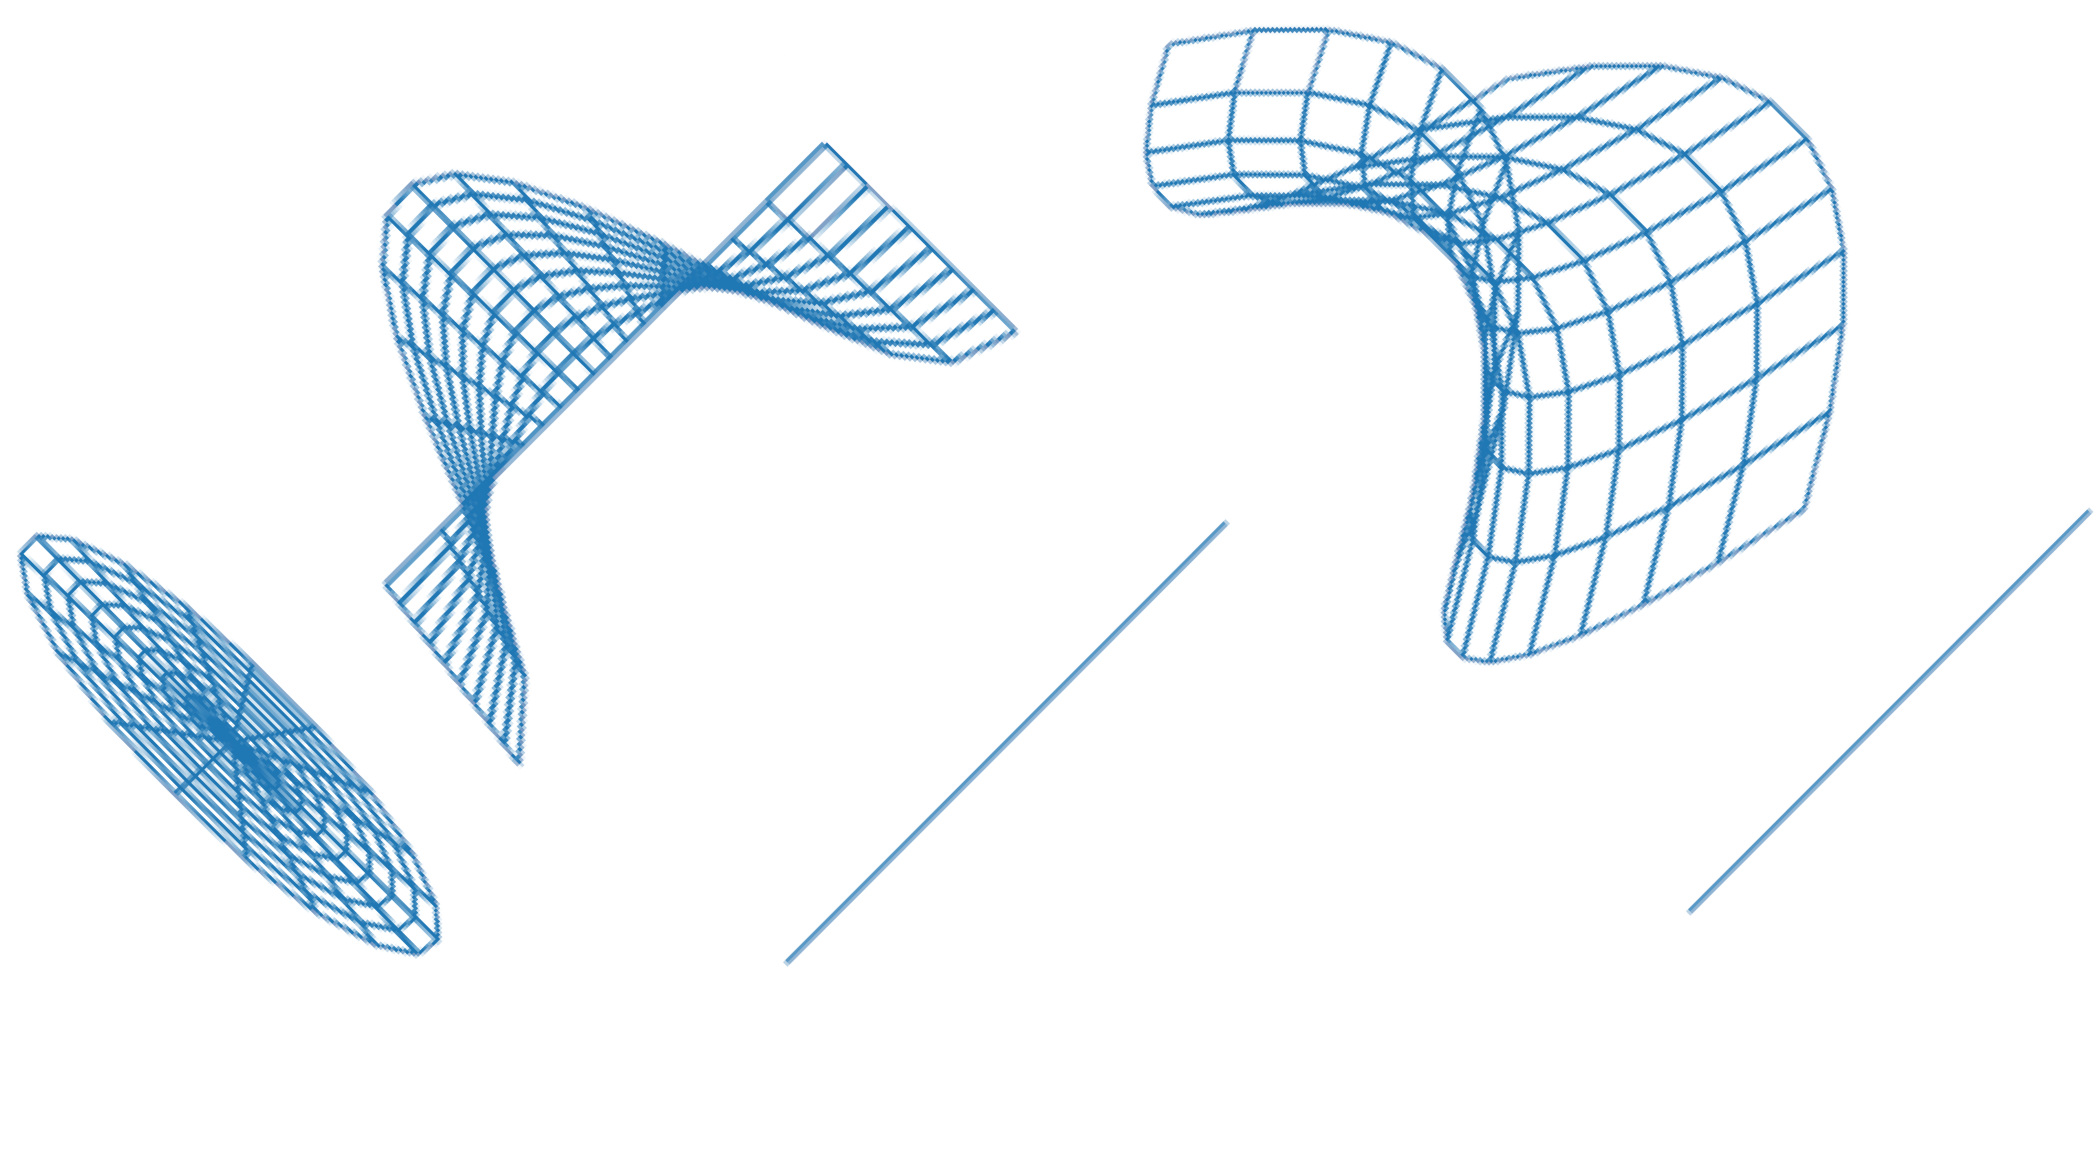
\includegraphics[scale=0.75]{Diagram.png}
					};
					
					
					%\draw (1,1) node [anchor=north west, inner sep=1pt]  [opacity=1 ,xscale=1.5,yscale=1.5]  {$S$}
					\draw (0,2.5) node [anchor=north east, inner sep=1pt]  [color=black ,opacity=1 ,xscale=3,yscale=3]  {$S$};
					
					\draw (-19,-17) node [anchor=north west, inner sep=1pt]  [color={rgb, 255:red, 208; green, 2; blue, 27 }  ,opacity=1 ,xscale=1.5,yscale=1.5]  {$\mathbb{P}^{2}$};
					
					\draw (-15,-5) node [anchor=south west, inner sep=1pt]  [color={rgb, 255:red, 208; green, 2; blue, 27 }  ,opacity=1 ,xscale=1.5,yscale=1.5]  {$\mathbb{F}_{1}$};
					
					\draw (15,0) node [anchor=north west, inner sep=1pt]  [color={rgb, 255:red, 208; green, 2; blue, 27 }  ,opacity=1 ,xscale=1.5,yscale=1.5]  {$\mathbb{P}^{1}\times \mathbb{P}^{1}$};
					
					\draw (0,-15) node [anchor=north west, inner sep=1pt]  [color={rgb, 255:red, 208; green, 2; blue, 27 }  ,opacity=1 ,xscale=1.5,yscale=1.5]  {$\mathbb{P}^{1}$};
					
					\draw (17,-15) node [anchor=north west, inner sep=1pt]  [color={rgb, 255:red, 208; green, 2; blue, 27 }  ,opacity=1 ,xscale=1.5,yscale=1.5]  {$\mathbb{P}^{1}$};
					
					
					%%Arrows
					
					\draw [-to, line width=1.5mm] (0,0.5) -- (2.5,-2) node[midway,sloped,above, xscale=1.5,yscale=1.5]  {$\pi_{3}$};
					
					\draw [-to, line width=1.5mm](-2,0.5) -- (-6,-3.5) node[midway,sloped,above, xscale=1.5,yscale=1.5]  {$\pi_{2}$};
					
					\draw [-to, line width=1.5mm](-12,-10.45) -- (-15,-13.40) node[midway,sloped,above, xscale=1.5,yscale=1.5]  {$\pi_{1}$} ;
					
					\draw [-to, line width=1.5mm](-8.5,-8.5) -- (-2.5,-14.5) node[midway,sloped,above, xscale=1.5,yscale=1.5]  {$\phi_{1}$};
					
					\draw [-to, line width=1.5mm](8,-6) -- (4,-10)  node[midway,sloped,above, xscale=1.5,yscale=1.5]  {$\phi_{2}$};
					
					\draw [-to, line width=1.5mm](13,-12) -- (15.5,-14.5) node[midway,sloped,above, xscale=1.5,yscale=1.5]  {$\phi_{3}$} ;
					\end{tikzpicture}
				\end{figure}
				
				
				
			\end{block}
			
			
			%\begin{alertblock}{Abundance Theorem}
			%Let $(X,B)$ be a klt threefold $R$-pair with $\mathbb{R}$-boundary. If $K_X+B$ is nef, then it is %semiample.
			%\end{alertblock}  
			
			
			
		\end{column}
		
		\separatorcolumn
		
		\begin{column}{0.44\paperwidth}
			
			\begin{block}{Geography of Ample Models - Definitions}
				Fix a $\mathbb{Q}$-divisor $A\geq 0$. Let $V$ be a finite dimensional, rational affine subspace of $WDiv_{\mathbb{R}}(X)$ containing no components of $A$. Such a $V$ is called a coefficient space (for A).
				
				We have the following.
				\[V_{A}= \{A+B: B \in V\}\]
				\[\mathcal{L}_{A}(V)=\{\Delta=A+B \in V_{A}: (X,\Delta) \text{ is klt}\}\]
				
				If $C \subseteq \mathcal{RL}_{A}(V)$ is a rational polytope then we have
				\[\mathcal{E}(C)=\{\Delta \in C: K_{X}+\Delta \text{ is pseudoeffective}\}\]
				
				Given a birational contraction $\phi:X \dashrightarrow Y$ we also define
				\[\mathcal{W}_{\phi}(C)=\{\Delta \in \mathcal{E}(C): \phi \text{ is a weak log canonical (wlc) model of } (X,\Delta)\}\]
				and given a rational map $\psi:X \dashrightarrow Z$ we have its ample class
				\[\mathcal{A}_{\phi}(C)=\{\Delta \in \mathcal{E}(C): \phi \text{ is the ample model of } (X,\Delta)\}\]
				
				Roughly speaking a wlc model is an output of the MMP. An ample model is the map induce by abundance from a wlc model.\\
				\hfill \break
				These definitions sweep some of the mxied characteristic specific difficulties. Rather than working with klt pairs, we have to work with rlt pairs. Roughly speaking this are pairs which can be replaced by a klt pair locally over a base. This is due to the lack of global Bertini type theorems.
				
			\end{block}
			
			\begin{alertblock}{Finiteness of Minimal Models}
				Let $X$ be a threefold over $R$. Let $C$ be a polytope inside $\mathcal{L}_{A}(V)$. Suppose there is a boundary $A+B \in \mathcal{L}_{A}(V)$ such that $(X,A+B)$ is a klt pair. Then the following hold:
				
				\begin{enumerate}
					\item There are finitely many birational contractions $\phi_{i}:X \dashrightarrow Y_{i}$ such that 
					\[\mathcal{E}(C) = \bigcup \mathcal{W}_{i}=\mathcal{W}_{\phi_{i}}(C)\]
					where each $\mathcal{W}_{i}$ is a rational polytope. Moreover if $\phi:X \to Y$ is a wlc model for any choice of $\Delta \in \mathcal{E}(C)$ then $\phi=\phi_{i}$ for some $i$, up to composition with an isomorphism.
					
					\item There are finitely many rational maps $\psi_{j}:X \dashrightarrow Z_{j}$ which partition $\mathcal{E}(C)$ into subsets $\mathcal{A}_{\psi_{j}}(C)=\mathcal{A}_{i}$.
					\item  For each $W_{i}$ there is a $j$ such that we can find a morphism $f_{i,j}: Y_{i} \to Z_{j}$ and $W_{i} \subseteq \overline{A_{j}}$.
					\item  $\mathcal{E}(C)$ is a rational polytope and $A_{j}$ is a union of the interiors of finitely many rational polytopes.
				\end{enumerate}
			\end{alertblock}
			
			\begin{block}{Application: Sarkisov Program}
				If $f:X \to Z$, $g:Y \to W$ are two Mori Fibre Spaces, a Sarkisov link $s:X \dashrightarrow Y$ is one the following.
				
				\[\begin{tikzcd}
				X' \arrow[d] \arrow[r, dotted] \arrow[r, "I", phantom, bend left=49] & Y \arrow[d]  & X' \arrow[r, dotted] \arrow[d] \arrow[r, "II",phantom, bend left=49] & Y' \arrow[d] & X \arrow[r, dotted] \arrow[d] \arrow[r, "III", phantom, bend left=49] & Y' \arrow[d] & X \arrow[d] \arrow[rr, dotted] \arrow[rr, "IV",phantom, bend left] &   & Y \arrow[d]       \\
				X \arrow[d]                                                          & W \arrow[ld] & X \arrow[d]                                               & Y \arrow[d]  & Z \arrow[rd]                                              & Y \arrow[d]  & Z \arrow[rd, "p"]                                          &   & W \arrow[ld, "q"'] \\
				Z                                                                    &              & Z \arrow[r, equal]                                                         & W            &                                                           & W            &                                                            & T &                  
				\end{tikzcd} \]
				where
				\begin{itemize}
					\item The horizontal map is a sequence of flops (codimension 2 birational transformations) for this pair
					\item Every vertical morphism is a contraction
					\item If the target of a vertical morphism is $X$ or $Y$ then it is an extremal divisorial contraction
					\item Either $p,q$ are both Mori Fibre Spaces (this is type $IV_{m}$) or they are both small contractions (type $IV_{s}$)
				\end{itemize}
				
			\end{block}
			
			The idea here is exactly the same as the example. We find a roof $R$ dominating $X,Y$ and a polygon $C\subseteq \mathcal{L}_{A}(V)$ such that $X,Y$ correspond to ample classes its decomposition (called a \textbf{geography}). The Sarkisov links then correspond the boundaries between ample classes. That Finiteness of Minimal Models implies the Sarkisov program is essentially due to \cite{HMX13}, though a few modifications are need in mixed characteristic.
			
		\end{column}
		
		\separatorcolumn
	\end{columns}
\end{frame}

\end{document}
